\documentclass{beamer}

\usepackage[utf8x]{inputenc}
\usepackage[english]{babel}
\usepackage{svg}
\usepackage{ulem}
\usepackage{tabularx}
\usepackage{hhline}
\usepackage{xcolor}


% define theme with .sty file
\usetheme{Nico}


% set path to images
\graphicspath{{/home/nico/Bureau/DNA_project/images/}}
\setsvg{svgpath = images/}


\title{DNA project.}
\institute{Artilect}


\begin{document}

\begin{frame}
\titlepage
\end{frame}

\begin{frame}
\frametitle{bases \& acides aminés}
\begin{itemize}
	\item<1-> 4 bases codant l'ADN:\\
	\hspace{120pt} A T G C
	\item<2-> 3 bases (codon) $\to$ 1 acide aminé
	\item<3-> 20 acides aminés codant les protéines:\\
	\hspace{120pt} A C D E F G H I K L M\\
	\hspace{120pt} N P Q R S T V W Y
	\item<4-> première combinaison de bases ATG $\to$ M:\\
	\hspace{120pt} Signal START
	\item<5-> 3 combinaisons de bases:\\
	\hspace{120pt} Signal STOP
	
\end{itemize}
\end{frame}

\begin{frame}
\frametitle{Mécanisme}
\centering
	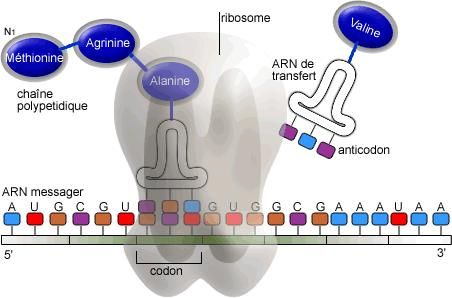
\includegraphics[width=\textwidth,height=0.5\textheight,keepaspectratio]{ribosome.jpg}
\end{frame}

\begin{frame}
\frametitle{Sequences}
\begin{overprint}
	\only<1>{
		\tiny
		$>$Homo sapiens hemoglobin, \textbf{DNA}\\~\\
		CATAAACCCTGGCGCGCTCGCGGCCCGGCACTCTTCTGGTCCCCACAGACTCAGAGAGAACCCACCATGG
		TGCTGTCTCCTGCCGACAAGACCAACGTCAAGGCCGCCTGGGGTAAGGTCGGCGCGCACGCTGGCGAGTA
		TGGTGCGGAGGCCCTGGAGAGGATGTTCCTGTCCTTCCCCACCACCAAGACCTACTTCCCGCACTTCGAC
		CTGAGCCACGGCTCTGCCCAGGTTAAGGGCCACGGCAAGAAGGTGGCCGACGCGCTGACCAACGCCGTGG
		CGCACGTGGACGACATGCCCAACGCGCTGTCCGCCCTGAGCGACCTGCACGCGCACAAGCTTCGGGTGGA
		CCCGGTCAACTTCAAGCTCCTAAGCCACTGCCTGCTGGTGACCCTGGCCGCCCACCTCCCCGCCGAGTTC
		ACCCCTGCGGTGCACGCCTCCCTGGACAAGTTCCTGGCTTCTGTGAGCACCGTGCTGACCTCCAAATACC
		GTTAAGCTGGAGCCTCGGTGGCCATGCTTCTTGCCCCTTGGGCCTCCCCCCAGCCCCTCCTCCCCTTCCT
		GCACCCGTACCCCCGTGGTCTTTGAATAAAGTCTGAGTGGGCGGCAAAAAAAAAAAAAAAAAAAAAA\\
		\vspace{20pt}
		
		$>$Homo sapiens hemoglobin, \textbf{amino acids}\\
MVLSPADKTNVKAAWGKVGAHAGEYGAEALERMFLSFPTTKTYFPHFDLSHGSAQVKGHGKKVADALTNA
VAHVDDMPNALSALSDLHAHKLRVDPVNFKLLSHCLLVTLAAHLPAEFTPAVHASLDKFLASVSTVLTSKYR
		}
	\only<2>{
		\tiny
		$>$Homo sapiens hemoglobin, \textbf{DNA}\\~\\
		CATAAACCCTGGCGCGCTCGCGGCCCGGCACTCTTCTGGTCCCCACAGACTCAGAGAGAACCCACC\textcolor{teal}{ATG}\textcolor{blue}{G
		TGCTGTCTCCTGCCGACAAGACCAACGTCAAGGCCGCCTGGGGTAAGGTCGGCGCGCACGCTGGCGAGTA
		TGGTGCGGAGGCCCTGGAGAGGATGTTCCTGTCCTTCCCCACCACCAAGACCTACTTCCCGCACTTCGAC
		CTGAGCCACGGCTCTGCCCAGGTTAAGGGCCACGGCAAGAAGGTGGCCGACGCGCTGACCAACGCCGTGG
		CGCACGTGGACGACATGCCCAACGCGCTGTCCGCCCTGAGCGACCTGCACGCGCACAAGCTTCGGGTGGA
		CCCGGTCAACTTCAAGCTCCTAAGCCACTGCCTGCTGGTGACCCTGGCCGCCCACCTCCCCGCCGAGTTC
		ACCCCTGCGGTGCACGCCTCCCTGGACAAGTTCCTGGCTTCTGTGAGCACCGTGCTGACCTCCAAATACC
		GT}\textcolor{red}{TAA}GCTGGAGCCTCGGTGGCCATGCTTCTTGCCCCTTGGGCCTCCCCCCAGCCCCTCCTCCCCTTCCT
		GCACCCGTACCCCCGTGGTCTTTGAATAAAGTCTGAGTGGGCGGCAAAAAAAAAAAAAAAAAAAAAA\\
		\vspace{20pt}
		
		$>$Homo sapiens hemoglobin, \textbf{amino acids}\\
\textcolor{teal}{M}\textcolor{blue}{VLSPADKTNVKAAWGKVGAHAGEYGAEALERMFLSFPTTKTYFPHFDLSHGSAQVKGHGKKVADALTNA
VAHVDDMPNALSALSDLHAHKLRVDPVNFKLLSHCLLVTLAAHLPAEFTPAVHASLDKFLASVSTVLTSKYR}
		}					
\end{overprint}
\end{frame}

\begin{frame}
\frametitle{Genetic code}
\centering
	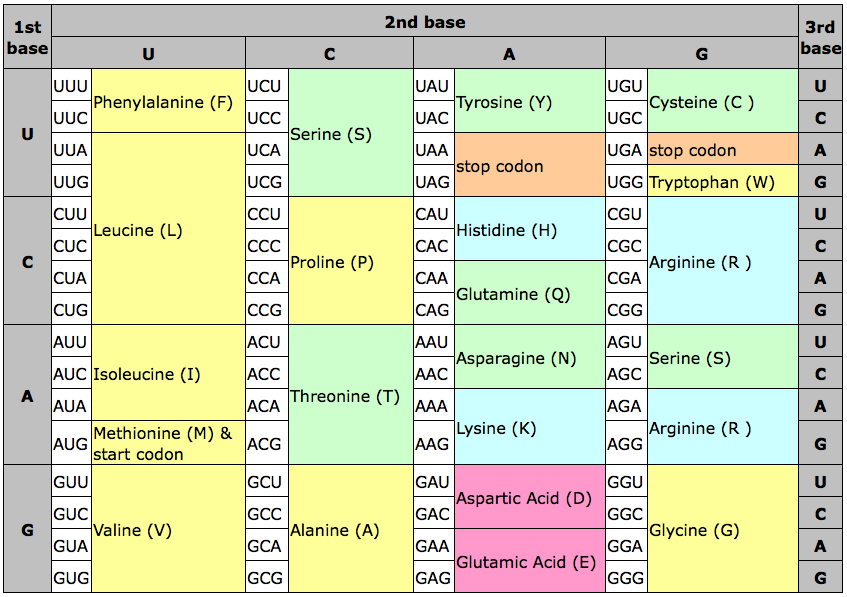
\includegraphics[width=\textwidth,height=0.5\textheight,keepaspectratio]{geneticCode.png}
\vspace{10pt}
\begin{overprint}
\onslide<1>
	\centering
	\begin{tabular}{|c|c|c|c|c|c|c|c|c|}
		\hline 
		\ldots & acc & \textcolor{teal}{ATG} & GTG & CTG & TCT & \ldots & \textcolor{red}{TAA} & ttc \\ 
		\hline 
		\ldots &  &  &  &  &  &  &  &  \\ 
		\hline 
	\end{tabular}	
\onslide<2>
	\centering
	\begin{tabular}{|c|c|c|c|c|c|c|c|c|}
		\hline 
		\ldots & acc & \textcolor{teal}{ATG} & GTG & CTG & TCT & \ldots & \textcolor{red}{TAA} & ttc \\ 
		\hline 
		\ldots & • &  &  &  &  &  &  &  \\ 
		\hline 
	\end{tabular}
\onslide<3>
	\centering
	\begin{tabular}{|c|c|c|c|c|c|c|c|c|}
		\hline 
		\ldots & acc & \textcolor{teal}{ATG} & GTG & CTG & TCT & \ldots & \textcolor{red}{TAA} & ttc \\ 
		\hline 
		\ldots & • & \textcolor{teal}{M} &  &  &  &  &  &  \\ 
		\hline 
	\end{tabular}
\onslide<4>
	\centering
	\begin{tabular}{|c|c|c|c|c|c|c|c|c|}
		\hline 
		\ldots & acc & \textcolor{teal}{ATG} & GTG & CTG & TCT & \ldots & \textcolor{red}{TAA} & ttc \\ 
		\hline 
		\ldots & • & \textcolor{teal}{M} & V &  &  &  &  &  \\ 
		\hline 
	\end{tabular}
\onslide<5>
	\centering
	\begin{tabular}{|c|c|c|c|c|c|c|c|c|}
		\hline 
		\ldots & acc & \textcolor{teal}{ATG} & GTG & CTG & TCT & \ldots & \textcolor{red}{TAA} & ttc \\ 
		\hline 
		\ldots & • & \textcolor{teal}{M} & V & L &  &  &  &  \\ 
		\hline 
	\end{tabular}
\onslide<6>
	\centering
	\begin{tabular}{|c|c|c|c|c|c|c|c|c|}
		\hline 
		\ldots & acc & \textcolor{teal}{ATG} & GTG & CTG & TCT & \ldots & \textcolor{red}{TAA} & ttc \\ 
		\hline 
		\ldots & • & \textcolor{teal}{M} & V & L & S &  &  &  \\ 
		\hline 
	\end{tabular}
\onslide<7>
	\centering
	\begin{tabular}{|c|c|c|c|c|c|c|c|c|}
		\hline 
		\ldots & acc & \textcolor{teal}{ATG} & GTG & CTG & TCT & \ldots & \textcolor{red}{TAA} & ttc \\ 
		\hline 
		\ldots & • & \textcolor{teal}{M} & V & L & S & \ldots &  &  \\ 
		\hline 
	\end{tabular}
\onslide<8>
	\centering
	\begin{tabular}{|c|c|c|c|c|c|c|c|c|}
		\hline 
		\ldots & acc & \textcolor{teal}{ATG} & GTG & CTG & TCT & \ldots & \textcolor{red}{TAA} & ttc \\ 
		\hline 
		\ldots & • & \textcolor{teal}{M} & V & L & S & \ldots & \textcolor{red}{X} &  \\ 
		\hline 
	\end{tabular}
\onslide<9>
	\centering
	\begin{tabular}{|c|c|c|c|c|c|c|c|c|}
		\hline 
		\ldots & acc & \textcolor{teal}{ATG} & GTG & CTG & TCT & \ldots & \textcolor{red}{TAA} & ttc \\ 
		\hline 
		\ldots & • & \textcolor{teal}{M} & V & L & S & \ldots & \textcolor{red}{X} & • \\ 
		\hline 
	\end{tabular}
\end{overprint}
\end{frame}

\begin{frame}
\frametitle{Fréquence de codage des AA}
\begin{tabular}{|c|c|c|c|c|c|c|c|c|c|c|}
\hline 
Acide Aminé & L & R & V & S & P & T & A & G & I & \textcolor{red}{X}\\ 
\hline 
Nb codons & 6 & 6 & 4 & 4 & 4 & 4 & 4 & 4 & 3 & 3\\ 
\hline 
\end{tabular}\\
\vspace{30pt}
\begin{tabular}{|c|c|c|c|c|c|c|c|c|c|c|c|}
\hline 
Acide Aminé & Y & H & Q & N & K & D & E & C & S & \textcolor{teal}{M} & W \\ 
\hline 
Nb codons & 2 & 2 & 2 & 2 & 2 & 2 & 2 & 2 & 2 & 1 & 1 \\ 
\hline 
\end{tabular} 


\end{frame}

\end{document}